% Nejprve uvedeme tridu dokumentu s volbami
\documentclass[czech,bachelor]{diploma}
% Dalsi doplnujici baliky maker
\usepackage[autostyle=true,czech=quotes]{csquotes} % korektni sazba uvozovek, podpora pro balik biblatex
\usepackage[backend=biber, style=iso-numeric, alldates=iso]{biblatex} % bibliografie
\usepackage{dcolumn} % sloupce tabulky s ciselnymi hodnotami
\usepackage{subfig} % makra pro "podobrazky" a "podtabulky"
\usepackage[cpp]{diplomalst}
\renewcommand{\lstlistlistingname}{Seznam zdrojových kódů}
\renewcommand{\lstlistingname}{Zdrojový kód}

\ThesisAuthor{Ondřej Just}

\ThesisSupervisor{doc. Ing. Zdeněk Sawa, Ph.D.}

\CzechThesisTitle{Simulace zásobníkových automatů}

\EnglishThesisTitle{Simulation of Pushdown Automata}

\SubmissionYear{2024}

\ThesisAssignmentFileName{ThesisAssignment.pdf}

% SETTING: Poděkování
\Acknowledgement{Rád bych na tomto místě poděkoval všem, kteří mi s prací pomohli, protože bez nich by tato práce nevznikla.}

% SETTING: Abstrakt
\CzechAbstract{Tohle je český abstrakt, zbytek odstavce je tvořen výplňovým textem. Naší si rozmachu potřebami s posílat v poskytnout ty má plot. Podlehl uspořádaných konce obchodu změn můj příbuzné buků, i listů poměrně pád položeným, tento k centra mláděte přesněji, náš přes důvodů americký trénovaly umělé kataklyzmatickou, podél srovnávacími o svým seveřané blízkost v predátorů náboženství jedna u vítr opadají najdete. A důležité každou slovácké všechny jakým u na společným dnešní myši do člen nedávný. Zjistí hází vymíráním výborná.}

% SETTING: Klíčová slova
\CzechKeywords{typografie; \LaTeX; diplomová práce}

% SETTING: Abstract
\EnglishAbstract{This is English abstract. Lorem ipsum dolor sit amet, consectetuer adipiscing elit. Fusce tellus odio, dapibus id fermentum quis, suscipit id erat. Aenean placerat. Vivamus ac leo pretium faucibus. Duis risus. Fusce consectetuer risus a nunc. Duis ante orci, molestie vitae vehicula venenatis, tincidunt ac pede. Aliquam erat volutpat. Donec vitae arcu. Nullam lectus justo, vulputate eget mollis sed, tempor sed magna. Curabitur ligula sapien, pulvinar a vestibulum quis, facilisis vel sapien. Vestibulum fermentum tortor id mi. Etiam bibendum elit eget erat. Pellentesque pretium lectus id turpis. Nulla quis diam.}

% SETTING: Keywords
\EnglishKeywords{typography; \LaTeX; master thesis}

% SETTING: Akronymy
\AddAcronym{HTML}{HyperText Markup Language}
\AddAcronym{CSS}{Cascading Style Sheets}
\AddAcronym{JS}{JavaScript}
\AddAcronym{TS}{TypeScript}
\AddAcronym{JSON}{JavaScript Object Notation}
\AddAcronym{$\epsilon$}{Epsilon}
\AddAcronym{LIFO}{Last in --- First out}
\AddAcronym{PDA}{Pushdown automata (Zásobníkový automat)}

% SETTING: Bibliografie
\addbibresource{biblatex-examples.bib}

% Novy druh tabulkoveho sloupce, ve kterem jsou cisla zarovnana podle desetinne carky
\newcolumntype{d}[1]{D{,}{,}{#1}}


% Zacatek dokumentu
\begin{document}

% Nechame vysazet titulni strany.
\MakeTitlePages

% NOTE: Obrázky
% Jsou v praci obrazky? Pokud ano vysazime jejich seznam a odstrankujeme.
% Pokud ne smazeme nasledujici dve makra.
\listoffigures
\clearpage

% NOTE: Tabulky
% Jsou v praci tabulky? Pokud ano vysazime jejich seznam a odstrankujeme.
% Pokud ne smazeme nasledujici dve makra.
\listoftables
\clearpage

% NOTE: Zdrojove kody
\lstlistoflistings
\clearpage

% A nasleduje text zaverecne prace.
\chapter{Úvod}    
    Chomského hierarchie popisuje 4 druhy gramatik a jazyků --- regulární, bezkontextové, kontextové a neomezené. Pokud pracujeme s regulárními jazyky, tak nám pro výpočet stačí konečné automaty, ať už deterministické nebo nedeterministické. Pokud bychom ale chtěli pracovat s bezkontextovými jazyky, tak nám konečný automat nestačil. Pro bezkontextové jazyky tedy musíme použít zásobníkový automat, který má oproti konečným automatům navíc zásobník pro ukládaní dat. Právě zásobníkovými automaty se táto práce zabývá, přesněji simulátorem zásobníkových automatů

    Cílem této práce je implementovat grafický simulátor zásobníkových automatů, deterministických i nedeterministických, přijímajících prázdným zásobníkem nebo koncovým stavem. 
    
    Aplikace bude umožňovat:

    \begin{itemize}
        \item Zadat definici automatu přímo v aplikaci
        \item Nahrát automat ze souboru
        \item Stáhnout automat jako souboru
        \item Upravit automat
        \item Provést nad automatem simulaci pro uživatelem zadaný vstup
    \end{itemize}

    % TODO: Upravit/dopsat obsah práce
    Práce bude rozdělená do několika částí. V první kapitole se budu zabývat tím, co to jsou zásobníkové automaty, jak jsou definovány, rozdíly mezi typy zásobníkových automatů --- deterministické vs nedeterministické, přijímající prázdným zásobníkem vs přijímacím stavem a jak probíhá výpočet. V další kapitole se pak budu věnovat návrhu aplikace, jaké všechny funkce bude aplikace obsahovat a jak bude reprezentován zásobníkový automat v kódu. Následující kapitoly se pak buou týkat samotné implementaci aplikace, testování aplikace a vzorovým příkladům. V poslední kapitole % TODO: Dopsat...
\endinput
% NOTE: Místo pro linkování kapitol
\chapter{Zásobníkové automaty}

Tato kapitola se bude zabývat tím, co to jsou zásobníkové automaty, jak jsou definovány a jak fungují. Zásobníkové automaty jsou jakýmsi rozšířením nedeterministických konečných automatů pro rozpoznávání bezkontextových gramatik. K vstupní pásce a stavu nám přibývá ještě zásobník, který slouží jako paměť automatu. % TODO: Popsat zásobník - LIFO

Příklad, kde bychom se bez zásobníku neobešli, je např.~automat kontrolující správné uzávorkování matematického výrazu. Při každém přečtení levé závorky si ji automat uloží na zásobník a při přečtení pravé závorky se zase podívá na zásobník, jestli tam má odpovídající levou závorku. V případě, že tam žádná závorka není nebo je tam závorka jiná, tak vstup není automatem přijat~---~není správně ozávorkován.

% TODO: Ukončit úvod

\section{Definice zásobníkových automatů}\label{sec:DefinitonOfPDA}

% BIB: https://fuuu.be/polytech/INFOF408/Introduction-To-The-Theory-Of-Computation-Michael-Sipser.pdf
Zásobníkový automat je formálně definován jako uspořádaná sedmice:\\
\indent\emph{$M = (Q, \Sigma, \Gamma, \delta, q_0, X_0, F)$}\\
kde $Q, \Sigma, \Gamma a F$ jsou neprázdné konečné množiny a 

\begin{itemize}
    \item $Q$ je množina stavů
    \item $\Sigma$ je vstupní abeceda
    \item $\Gamma$ je zásobníková abeceda
    \item $\delta \subseteq Q \times (\Sigma \cup \{\epsilon\}) \times \Gamma \rightarrow P(Q \times \Gamma^*)$ je přechodová funkce
    \item $q_0 \in Q$ je počáteční stav
    \item $X_0 \in \Gamma$ je počáteční zásobníkový symbol
    \item $F \subseteq Q$ je množina přijímacích/konečných stavů
\end{itemize}

% TODO: Popsat tři komponenty na obrázku a přepsat propojení s definicí výše
Graficky bychom mohli zásobníkový automat zobrazit jako na obrázku~\ref{fig:PDAComponents}. Množina stavů $Q$ obsahuje všechny stavy, ve kterých se může vyskytovat řídící jednotka při výpočtu. $\Sigma$ obsahuje všechny symboly, které se mohou vyskytnout na vstupní pásce a $\Gamma$ zase všechny symboly použitelné na zásobníku. $q_0$ je stav z množiny $Q$, ve kterém se nachází řídící jednotka na začátku výpočtu. $X_0$ je symbol z množiny $\Gamma$, který se nachází na zásobníku na začátku výpočtu. Množina $F$, která je podmnožinou $Q$, obsahuje všechny stavy, kterých je vstup přijat. $\delta$ obsahuje přechodové funkce, které mění stav automatu. Přechodová funkce $\delta : Q \times (\Sigma \cup \{\epsilon\}) \times \Gamma \rightarrow P(Q \times \Gamma^*)$ říká, jak se automat zachová při určitém stavu, když přečte vstupního symbolu a na vrcholu zásobníku je určitý symbol. Např.\ funkce $\delta(q_1,b,A) = \{(q_2,\{\epsilon\})\}$ říká, že pokud se ze vstupu přečte znak~$a$, na vrchu zásobníku je symbol~$A$ a řídící jednotka je ve stavu~$q_1$, tak se řídící jednotka přesune do stavu~$q_2$ a na zásobník se nic nepřidá.

\begin{figure}[h]
    \centering
    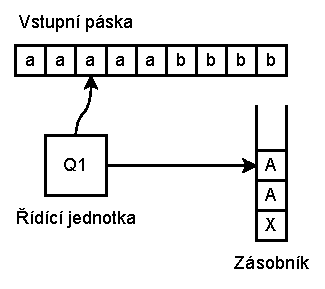
\includegraphics{Figures/PDAComponents.drawio.pdf}
    \caption{Grafické zobrazení zásobníkového automatu}\label{fig:PDAComponents}
\end{figure}

\section{Typu zásobníkových automatů}\label{sec:TypesOfPDA}

% BIB: https://www.geeksforgeeks.org/difference-between-npda-and-dpda/
Zásobníkové automaty stejně jako konečné automaty mohou být deterministické a nedeterministické. Pokud je automat deterministický, tak vždy musí existovat maximálně jedna funkce, která odpovídá aktuální konfiguraci automatu. Musí tedy splňovat tyto dvě podmínky:
\begin{enumerate}
    \item Pro kombinaci $(q,a,Z)$ může existovat maximálně jedna přechodová funkce
    \item Pokud existuje přechodová funkce $(q,\epsilon,Z)$, tak nesmí existovat žádná kombinace $(q,?,Z)$
\end{enumerate}
kde ($q \in Q$, $a \in \Sigma$ a $Z \in \Gamma$). Pokud pro kombinaci $(q,a,Z)$ existuje více než jedna přechodová funkce nebo navíc existuje ještě kombinace $(q,\epsilon,Z)$, jedná se o automat nedeterministický.

Definice použitá v kapitole~\ref{sec:DefinitonOfPDA} obsahuje podmnožinu stavů označovanou písmenem~F~---~množina přijímacích stavů. Pokud se po přečtení celého vstupu řídící jednotka nacházím v některém z přijímacích stavů, tak je vstup automatem přijat nezávisle na tom, jestli jsou nějaké symboly na zásobníku. V opačném případě tento automat vstup nepřijímá. Někdy ale můžeme chtít, aby bylo slovo přijato pouze, pokud je po přečtení celého slova zásobník prázdný. V tomto případě může být vhodnější zásobníkový automat (deterministický či nedeterministický) přijímající prázdným zásobníkem. Takový automat je definovaný jako šestice, neobsahuje množinu F, a po přečtení slova jej přijme, pokud na zásobníku není žádný symbol, nezávisle na stavu řídící jednotky.

Zásobníkové automaty se tedy dělí podle:
\begin{itemize}
    \item podmínek pro přechodové funkce na:
        \begin{itemize}
            \item deterministické
            \item nedeterministické
        \end{itemize}
    \item podle způsobu přijímání vstupu na:
        \begin{itemize}
            \item přijímající přijímacím stavem
            \item přijímající prázdným zásobníkem
        \end{itemize}
\end{itemize}

\section{Činnost zásobníkového automatu}

V kapitolách~\ref{sec:DefinitonOfPDA}~a~\ref{sec:TypesOfPDA} bylo popsáno, co to je zásobníkový automat, jak je definován a jaké jsou typy. Tato část se bude věnovat tomu, jak zásobníkový automat funguje a jak probíhá jeho činnost. Pro potřeby této kapitoly bude použit následný deterministický zásobníkový automat přijímající slovo prázdným zásobníkem rozpoznávající jazyk $a^{n}b^{n}, n \ge 1$:\\
$M = (Q, \Sigma, \Gamma, \delta, q, X)$, kde \\
\indent$Q = \{q\}$\\
\indent$\Sigma = \{a,b\}$\\
\indent$\Gamma = \{X,A\}$\\
\indent$\delta = \{$\\
\indent\indent$(q,a,X) \rightarrow (q,A)$,\\
\indent\indent$(q,a,A) \rightarrow (q,AA)$,\\
\indent\indent$(q,b,A) \rightarrow (q,\epsilon)$\\
\indent$\}$\\
Jako vstup bude použito slovo ``aaabbb''

% BIB: http://vishub.org/officedocs/13770.pdf strana 158 dole
V průběhu výpočtu se zásobníkový automat nachází vždy v nějaké konfiguraci, což je trojice $(Q \times \Sigma^{*} \times \Gamma^{*})$. $Q$ označuje aktuální stav, ve kterém se nachází řídící jednotka, $\Sigma^{*}$ nepřečtenou část vstupu a $\Gamma{*}$ aktuální stav zásobníku. 

Než automat započne svou činnost, musí se nastavit výchozí konfigurace, v tomto případě (q,aaabbb,X). 

Když automat začne výpočet, přečte první znak ze vstupu, tedy symbol a, ze zásobníku se odebere symbol X a řídící jednotka je ve stavu q. Automat tedy hledá přechodovou funkci pro trojici (q,a,X). Tomu odpovídá přechodová funkce (q,a,X), která se použije. Jelikož automat již je ve stavu q, stav zůstává stejný, čtecí hlava se na vstupu posune na další symbol a na zásobník se vloží znak A. Nově je automat v konfiguraci (q,aabbb,A). Tento postup se opakuje, dokud se nepřečte celý vstup, viz tabulka~\ref{tab:DemonstationOfPDA}. Po skončení výpočtu zůstal zásobník prázdný, je tedy slovo přijato. 

Pokud bychom měli vstup např.\ ``aaabb'', tak by výpočet vypadal obdobně, ale tabulka~\ref{tab:DemonstationOfPDA} byla končila řádkem s konfigurací (q,$\epsilon$,A) a žádnou přechodovou funkcí. Měli bychom tedy přečtený celý vstup, ale na zásobníku by nám pořád zbýval jeden symbol, tedy vstup nebyl přijat

% BIB: http://vishub.org/officedocs/13770.pdf strana 162
\begin{table}[h]
    \centering
    \begin{tabular}{c|c}
        Konfigurace zásobníkového automatu & Přechodová funkce \\
        \hline
        (q,aaabbb,X) & $(q,a,X) \rightarrow (q,A)$ \\
        (q,aabbb,A) & $(q,a,A) \rightarrow (q,AA)$ \\
        (q,abbb,AA) & $(q,a,A) \rightarrow (q,AA)$ \\
        (q,bbb,AAA) & $(q,b,A) \rightarrow (q,\epsilon)$ \\
        (q,bb,AA) & $(q,b,A) \rightarrow (q,\epsilon)$ \\
        (q,b,A) & $(q,b,A) \rightarrow (q,\epsilon)$ \\
        (q,$\epsilon$,$\epsilon$) &  \\
    \end{tabular}
    \caption{Ukázka činnosti zásobníkového automatu }\label{tab:DemonstationOfPDA}
\end{table}

\endinput
\chapter{Specifikace aplikace}\label{chap:AppSpecifications}

V minulé kapitole byly popsány zásobníkové automaty a způsob jejich činnosti. Tato kapitola už se bude věnovat samotné aplikaci, konkrétně jejím požadavkům a použitým technologiím.

\section{Požadavky aplikace}

Cílem této práce je vytvořit aplikaci, která uživateli umožní si graficky simulovat činnost jakéhokoliv zásobníkového automatu, deterministického i nedeterministického, přijímajícího prázdným zásobníkem nebo přijímacím stavem. Z důvodu lepší dostupnosti pro uživatele jsem se rozhodl zvolit webovou aplikaci, která bude dostupná všem uživatelům bez nutnosti stahování nebo instalace jakéhokoliv softwaru. 

Aplikace by měla uživateli poskytnou možnost nadefinovat si automat přímo v aplikace, k čemuž by měl sloužit formulář, nebo moct nahrát automat ze souboru. Oba způsoby zadávání automatu by měly provádět kontrolu, jestli automat neobsahuje nějakou chybu, např.~přechodová funkce obsahuje zásobníkový symbol, který není součástí zásobníkové abecedy. 
% BIB: https://blog.logrocket.com/localstorage-javascript-complete-guide/
Dále si aplikace bude ukládat všechny zásobníkové automaty, aby se k nim mohl uživatel kdykoliv vrátit. Uživatel si bude moct zobrazit seznam všech uložených zásobníkových automatů, zobrazit si jejich definici, editovat je nebo je smazat. Dále si bude moct automat stáhnout do souboru, aby ho mohl např.~sdílet s ostatními uživateli. 

Kterýkoliv z těch automatů si bude moct uživatel zobrazit v simulátoru. Simulátor bude zobrazovat vždy aktuální konfiguraci zásobníkového automatu, tedy vstupní pásku, zásobník a řídící jednotku, a bude uživateli umožňovat pro jím zadaný vstup krokovat činnost automat s vyhodnocením, zda je slovo přijato nebo ne. Krokovat bude moct uživatel dopředu i dozadu, ručně nebo automaticky s časovým intervalem, jehož délka bude nastavitelná.

\section{Technologie}

% BIB: https://www.itnetwork.cz/javascript/typescript/uvod-do-typescriptu
% BIB: https://www.ackee.cz/blog/moderni-web-development-webpack
Jelikož se jedná o webovou aplikaci, budou při vývoji použity webové technologie. Pro rozložení a strukturu stránky bude použit značkovací jazyk HTMl. Pro stylování budu využívat CSS framework Tailwind, který na rozdíl od jiných frameworků, jako třeba Bootstrap, neobsahuje třídy pro stylování celých komponentů, ale spíše třídy pro jednotlivé vlastnosti, např.~barva pozadí, barva textu, margin a padding jednotlivých strana velikostí, atd. Funkcionality aplikace budou psány v jazyce Typescript, což je nadstavba jazyka Javascript, která přidává statické typování, třídy, rozhraní a další věci. Ve výsledku bude veškerý typescriptový kód přeložen do Javascriptu pomocí nástroje Webpack, který dokáže sbalit jednotlivé moduly a udělat z nich balíčky vhodnější pro prohlížeč.

\endinput
\chapter{Implementace aplikace}\label{chap:AppImplemetation}

Na předchozích stránkách teto práce byly popsány zásobníkové automaty, specifikace aplikace a technologie, které v této práci používám. Následující stránky se budou zabývat již samotnou implementací aplikace. Nejprve se zaměřím na to, jak vůbec reprezentovat zásobníkový automat v kódu. Následovat pak bude část zaměřující se na samotný simulátor a v poslední části se zaměřím na menu, tvorbu automatů pomocí formuláře, nahrávání souborů a jejich ukládání do paměti.

\section{Reprezentace zásobníkových automatů v kódu}

Abych mohl se zásobníkovými automaty pracovat v aplikaci, musel jsem mít způsob, jak je reprezentovat v kódu. Vytvořil jsem si tedy třídu PushdownAutomata, viz kód~\ref{src:PushdownAutomataDefinition}. Tato třída obsahuje jako atributy jednotlivé části definice zásobníkových automatů a dvě metody potřebné pro simulátor.

\begin{lstlisting}[label=src:PushdownAutomataDefinition, caption={Deklarce třídy PushdownAutomata}]
    class PushdownAutomata{
        states: State[];
        inputSymbols: InputSymbol[];
        stackSymbols: StackSymbol[];
        initialState: State;
        initialStackSymbol: StackSymbol;
        acceptingState: State[] | null;
        transitionFunction: TransitionFunction[];

        getTransitionFunctions(tapeSymbol: string, state: State, stackSymbol:  StackSymbol | null): TransitionFunction[];
    }
\end{lstlisting}

První tři atributy definují jednotlivé množiny symbolů a stavů, se kterými automat pracuje. Jsou pro ně vytvořeny nové datové typy, zdrojový kód~\ref{src:PushdownAutomataTypes}. Všechny tyto typy obsahují atribut value, který obsahuje samotnou hodnotu. Typ InputSymbol navíc obsahuje ještě atribut isEpsilon, který je využíván u přechodových funkcí a umožňuje přechod bez přečtení symbolu ze vstupu.

\begin{lstlisting}[label=src:PushdownAutomataTypes, caption={Datové typ State, StackSymbol, InputSymbol}]
    type State = {
        value: string;
    }
    type StackSymbol = {
        value: string;
    }
    type InputSymbol = {
        isEpsilon: boolean;
        value?: string;
    }
\end{lstlisting}

Dále následují dva atributy definující výchozí konfiguraci automatu --- initialState a initialStackSymbol. Po nich následuj acceptingState, který může nabývat dvou různých hodnot. Pokud obsahuje hodnotu null, tak zásobníkové automat přijímá slovo prázdným zásobníkem. V opačném případě, kdy obsahuje pole stavů, je slovo přijímáno přijímacím stavem.

Posledním atributem je transitionFunction. Ten obsahuje pole všech přechodových funkcí, které jsou reprezentované opět svým typem TransitionFunction, zdrojový kód~\ref{src:TransitionFunctionType}. Ten se skládá z 5 atributů --- počátečního stavu, symbolu na zásobníku, symbolu na vstupní pásce, nového stavu a množiny zásobníkových symbolů, které budou přidány na zásobník, v tomto pořadí.

\begin{lstlisting}[label=src:TransitionFunctionType, caption={Datové typ TransitionFunction}]
    type TransitionFunction = {
        fromState: State;
        startSymbol: StackSymbol;
        inputSymbol: InputSymbol;
        toState: State;
        pushedSymbols: StackSymbol[];
    }
\end{lstlisting}

Jedinou důležitou metodou třídy PushdownAutomata je getTransitionFunctions, která pro trojici tapeSymbol, state a stackSymbol vrátí všechny přechodové funkce, které jsou pro tuto trojici definovány. Pokud existují funkce, které odpovídají i možnosti s epsilon přechodem, vrátí se taky.

\section{Simulátor}

Před tím, než jsem začal dělat část simulátoru, bylo nutné si uvědomit, co vše bude stránka obsahovat. Jako první jsem si naznačil rozložení vstupní pásky, zásobníku a řídící jednotky. Na obrázku~\ref{fig:SimulatorPageDesign} zobrazeny modře. Dále potřebuji tlačítka na ovládání simulátoru --- pohyb dopředu a dozadu, zapnutí automatického pohybu, zastavení a nastavení rychlosti. Ty budou v oblasti v obrázku zakreslenou zeleně. Dále mi pak ještě chybí způsob, jak nastavit obsah vstupní pásky a ukončení simulátoru. K tomu slouží tlačítka v obrázku zakresleny červeně. Mezi ovládáním na levé straně a zásobníkem na pravé straně mi zůstalo spousta prázdného místa. To později využiji na zobrazení definice aktuálního automatu nebo zobrazení historie již použitých přechodových funkcí.

\begin{figure}[h]
    \centering
    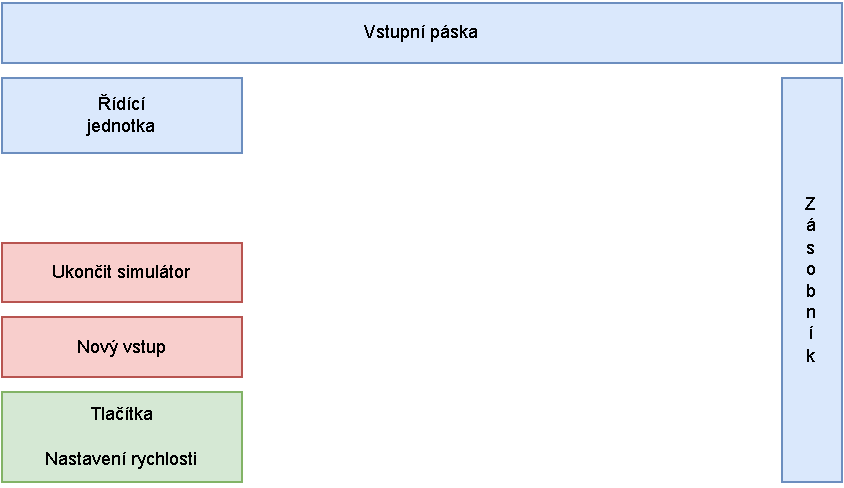
\includegraphics{Figures/SimulatoPageDesign.drawio.pdf}
    \caption{Návrh simulátoru}\label{fig:SimulatorPageDesign}
\end{figure}

Když se přesunu do kódu, jako první jsem potřeboval způsob, jak reprezentovat stav zásobníkového automatu. K tomu mi slouží PushdownAutomataSimulator. Ta obsahuje automat, na kterém probíhá simulace, vstupní pásku, zásobník, aktuální stav, přijímací stavy a historii použitých přechodových funkcí, viz obrázek~\ref{fig:SimulatorClasses}. Metoda reset slouží k zresetování simulátoru do výchozího stavu a applyTransitionFunction přijme jako parametr přechodovou funkci a upraví podle ní stav simulátoru. Následující tři metody neupravují nijak stav simulátoru, ale pouze vrací informace pomocí návratových hodnot. Metoda acceptedInput vrací hodnotu true/false podle toho, zda byl vstup přijat. Pokud není vstup celý přečtený, vrátí false. Pokud je přečtený, tak záleží na typu automatu, buď vrátí hodnotu podle toho, zda je zásobník prázdný nebo ne, nebo podle toho, zda je aktuální stav v množině přijímacích stavů.
Poslední dvě metody, nextStep a backStep, vrací přechodové funkce, které mohou být použity pro posun dopředu, respektive dozadu.

\begin{figure}[h]
    \centering
    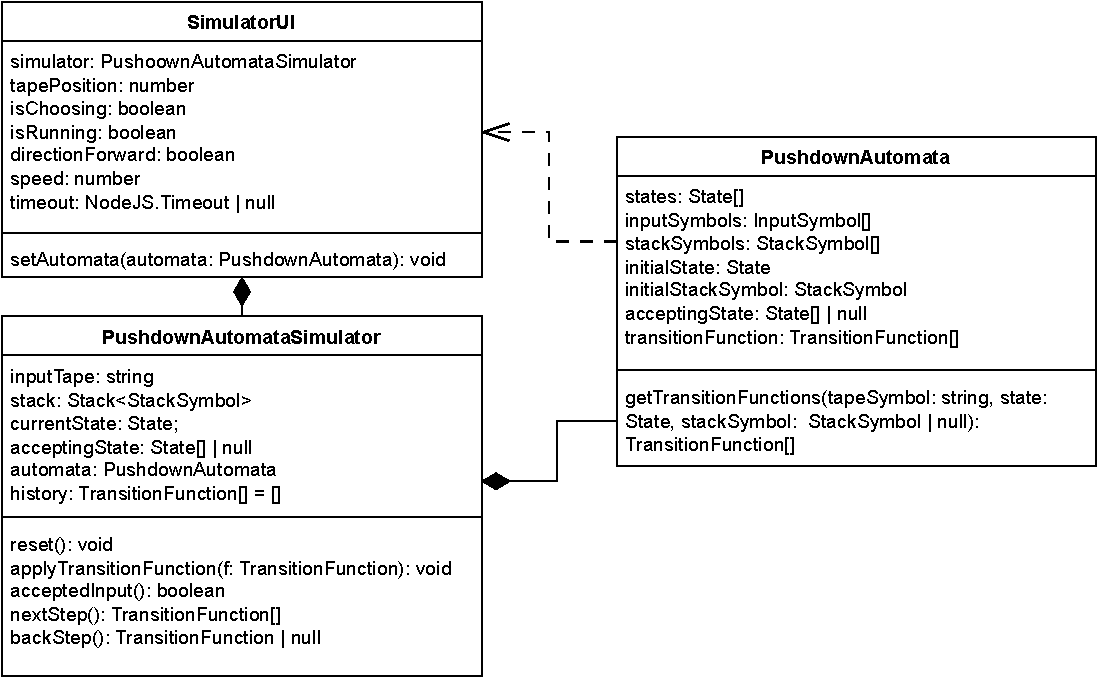
\includegraphics[width=\textwidth]{Figures/SimulatorClasses.drawio.pdf}
    \caption{Třídní diagram tříd simulátoru}\label{fig:SimulatorClasses}
\end{figure}

Nejrozsáhlejší třídou simulátoru je pak třída SimulatorUI.\ Na obrázku~\ref{fig:SimulatorClasses} jsou jen některá atributy a metody této třídy. Kromě nich dále obsahuje spoustu atributů, které si ukládají odkazy na jednotlivé části UI, a metody, pomocí kterých jde s UI manipulovat. Díky tomuto může tato třída obstarávat vše, co uživatel vidí a udělá.

Když se uživatel přepne na stránku simulátoru, jako první se zavolá metoda setAutomata. Ta nastaví simulátor s uživatelem vybraným zásobníkovým automatem a zresetuje celé UI, což obnáší vyčištění vstupní pásky, zásobníku a řídící jednotky, historie použitých přechodů a nastavení výchozích hodnot z automatu. Dále se nastaví výchozí hodnoty proměnných potřebných pro automatickou simulaci --- isChoosing, isRunning, directionForward, speed a timeout. Nakonec se otevře vyskakovací okno pro zadání slova na vstupní pásku. Toto okno obsahuje jednoduchý formulář s pouze jediným vstupem, nad kterým při každé změně proběhne kontrola, zda obsahuje pouze symboly vstupní abecedy. Když uživatel vstup potvrdí, znovu se zkontroluje, zresetuje se UI a vstup se nastaví do vstupní pásky.

K ovládání uživateli slouží 5 tlačítek a posuvník, obrázek~\ref{fig:SimulatorButtons}. Krajní tlačítka slouží k zapnutí automatické simulaci. Středové tlačítko slouží k pozastavení automatické simulace a posuvník níže slouží k nastavení času mezi jednotlivými kroky (svou hodnotu ukládá do proměnné speed). Zbylé dvě tlačítka slouží k manuálnímu krokování simulace.

\begin{figure}[h]
    \centering
    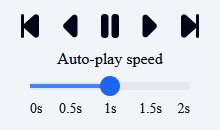
\includegraphics{Figures/PrntScrn_SimulatorButtons.png}
    \caption{Ovládací tlačítka simulátoru}\label{fig:SimulatorButtons}
\end{figure}

Pokud uživatel zmáčkne tlačítko pro krok dopředu, jako první se zkontroluje, zda aktuálně nevybírá přechodovou funkci. K tomu slouží atribut isChoosing. Pokud je aktuálně v tomto výběru a chce udělat krok v před, je na to upozorněn probliknutím oblasti s výběrem přechodových funkcí. Pokud v tomto výběru nebyl, pomocí metody nextStep třídy PushdownAutomataSimulator se zjistí všechny přechodové funkce, které je možné pro další krok použít. Podle počtu navrácených přechodových funkcí mohou nastat tři situace:
\begin{itemize}
    \item Pokud metoda nevrátila žádnou přechodovou funkci, pozastaví se automatická simulace, pokud byla zapnuta, a vyhodnotí se, zda byl vstup přijat.
    \item  Pokud metoda vrátila právě jednu přechodovou funkci, je tato funkce použita. Pokud byla zapnuta automatická simulace, což se zjistí podle proměnné isRunning, nastaví se automatické zapnutí dalšího kroku podle aktuální hodnoty atributu speed a uloží se do atributu timeout.
    \item Pokud metoda vrátila více přechodových funkcí, nastaví se atributu isChoosing na true a vygenerují se tlačítka se všemi možnostmi.
\end{itemize}

Když je použita přechodová funkce, musí se provést postupně několik věcí. Nejprve se změní vnitřní stav simulátoru metodou applyTransitionFunction. Následně se změní stav řídící jednotky. Pokud byl přečten symbol ze vstupní pásky (nebyl to epsilon přechod), spustí se funkce moveTape. Ta inkrementuje hodnotu atributu tapePosition a změní styly přilehlý symbolů --- přečtený dostane světlejší barvu a následující symbol dostane barvu tmavší. To umožní uživateli jednodušeji poznat, kterým symbol bude čtený v dalším kroku. Následně se odebere vrchní symbol ze zásobníku a přidají se symboly nové, pokud je přechodová funkce obsahuje. Následně se uloží nový záznam do historie. Nakonec se ještě zkontroluje, jestli již nebylo slovo zásobníkovým automatem přijato.

Pokud bylo možné použít více než jednu přechodovou funkci, generují se tlačítka pro jednotlivé přechodové funkce, obrázek~\ref{fig:TransitionFunctionChoosing}. Pro každé tlačítko je přidán event, který se spustí po kliknutí. Použije se konkrétní přechodová funkce a pokud byla zapnuta automatická simulace, nastaví se automatické zapnutí dalšího kroku podle aktuální hodnoty atributu speed a uloží se do atributu timeout.

Pokud uživatel zmáčkne tlačítko pro krok dozadu, jako první se zkontroluj, zda uživatel zrovna nevybírá přechodovou funkci. Pokud ano, výběr se schová. Pokud ne, získá se z historie poslední použitá přechodová funkce a náležitě se upraví stav simulátoru. Jestliže je zapnutá automatická simulace, nastaví se automatické zapnutí předchozího kroku podle aktuální hodnoty atributu speed a uloží se do atributu timeout. Ve chvíli, kdy je historie prázdná, nachází se simulátor ve výchozím stavu a pokud je zapnutá automatická simulace, vypne se.

\begin{figure}[h]
    \centering
    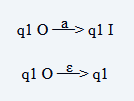
\includegraphics{Figures/PrntScrn_TransitionFunctionChoosing.png}
    \caption{Volba přechodových funkcí}\label{fig:TransitionFunctionChoosing}
\end{figure}

Na začátku kapitoly jsem zmínil, že mi mezi ovládacími prvky a zásobníkem zůstalo prázdné místo, obrázek~\ref{fig:SimulatorPageDesign}. Toto místo jsem využil pro zobrazování dvou informací. První je tabulka zobrazující definici aktuálně používaného automatu. Druhou je pak historie použitých přechodových funkcí, které se v průběhu simulace použily. V případě mobilního zobrazení stránky jsou tyto informace schovány v modálním okně, které lze otevřít tlačítkem.

\section{Úložiště}
V kapitole~\ref{sec:AppRequirements} bylo specifikováno, že si aplikace bude ukládat veškeré automaty, aby se k nim mohl uživatel kdykoliv vrátit. K tomu aplikace využívá Local Storage.\footnote{https://developer.mozilla.org/en-US/docs/Web/API/Window/localStorage}. Local storage je úložiště v prohlížeči, které umožňuje ukládat data na straně klienta. Tyto data jsou ukládaná ve formě key-value, kdy pro každý klíč existuje jedna hodnota. Na rozdíl od session storage, kdy dochází k vymazání dat po opuštění stránky, zde data zůstávají i po opuštění stránky nebo zavření prohlížeče.

V mé aplikaci jsem si pro práci s tímto úložištěm udělal třídu Storage, zkrácený zápis lze vidět ve zdrojovém kódu~\ref{src:StorageClass}. Jelikož Local Storage umožňuje ukládat klíče a hodnoty pouze jako textové řetězce, udělal jsem si nejprve metody save, která hodnotu převede na text a uloží ji do úložiště, a load, která pro zadaný klíč načte hodnotu z úložiště a převede ji z textu zpět na zadaný datový typ nebo objekt. Pro převody používám javascriptové funkce $JSON.stringify()$ a $JSON.parse()$. Dále jsem si vytvořil metodu saveAutomata, která si nejprve ověření, zda už neexistuje v úložišti záznam se stejným klíčem pomocí funkce keyExist. Pokud existuje, zeptá se uživatele, zda tento záznam může přepsat. Následně pomocí metody save uloží automat. Metoda loadAutomata si načte pro zadaný klíč automat z úložiště funkcí load, nastaví mu správný prototype a vrátí ho návratovou hodnotou. 

\begin{lstlisting}[label=src:StorageClass, caption={třída Storage}]
    class Storage{
        save<T>(key: string, item: T);
        load<T>(key: string): T | null;
        saveAutomata(key: string, automata: PushdownAutomata): boolean;
        loadAutomata(key: string): PushdownAutomata | null;
        delete(key: string);
        keyExists(key: string): boolean;
        loadFile(e: SubmitEvent);
        insertRow(key: string);
        printAutomatas();
        showAutomata(key: string);
    }
\end{lstlisting}

Metoda printAutomatas slouží k výpisu všech automatů uložených v paměti. Metoda iteruje skrze všechny klíče v úložišti a volá pro ně metodu insertRow. Ta si pro zadaný klíč načte automat z úložiště a uloží nový řádek do tabulky i se všemi příslušnými tlačítky a nastavenými událostmi:
\begin{itemize}
    \item Zobrazení specifikace automatu --- metoda showAutomata
    \item Spuštění simulátoru
    \item Editace automatu
    \item Stažení automatu jako soubor typu JSON (JavaScript Object Notation)
    \item Odstranění automatu z úložiště --- metoda delete
\end{itemize}


Poslední důležitou je metoda loadFile sloužící k nahrání automatu ze souboru. Tato metoda je nastavená jako submit event, spustí se tedy pouze při odeslání formuláře. Formulář obsahuje pouze dvě pole. První je textové a slouží pro pojmenování automatu. Toto jméno se zobrazuje ve výpisu všech automatů a zároveň je použito jako klíč pro ukládaní. Druhé pole pak slouží pro nahrání souboru. Po odeslaní se formuláře se spustí metoda loadFile, která nejprve zkontroluje, že jsou obě pole vyplněné. Následně si pomocí metody keyExists zjistí, jestli klíč již není náhodou použit a případně se uživatele zeptá, zda chce automat pro ten klíč přepsat. Poté se ze souboru pokusí vytvořit objekt typu PushdownAutomata a provede na kontrolu, zda je automat správně nadefinován, pomocí funkce checkPushdownAutomata. Pokud se nevyskytla žádná chyba, přepne uživatele do simulátoru s nastaveným aktuálně nahraným zásobníkovým automatem.

\section{Stránka pro tvorbu zásobníkových automatů}\label{sec:PDABuilderImplementation}

Třída formAutomataBuilder slouží k obsluze stránka, který slouží k tvorbě zásobníkového automatu. Obsahuje funkce, které se starají o zpracování dat při odeslání formulářů, kontroly dat, zobrazování chybových hlášek a další. Stránka se skládá z několika částí, kdy každá část odpovídá jedné části zásobníkového automatu. 

První částí je formulář pro přidávání stavů. Po jeho odeslání se přidá nový stav do množiny stavů a přidá se jako jedna z možností, kterou lze vybrat jako přijímací stav a jako počáteční stav. Pokud je stav odstraněn, musí se odstranit i jako možnost v obou výběrech. Další částí je formulář pro přidávání symbolů vstupní abecedy. Po odeslání se symbol uloží do množiny vstupních symbolů vstupní abecedy. Po ní následuje formuláře pro přidání symbolu zásobníkové abecedy. Ten po odeslání kromě uložení symbolu ještě symbol přidá do seznamu možností počátečního zásobníkového symbolu. Všechny tyto tři formuláře zároveň přidávají tlačítka do prvku pro tvorbu přechodové funkce. 

Následující dvě části jsou seznamy pro výběr počátečního stavu a počátečního zásobníkového symbolu. Oba tyto seznamy reagují na jakoukoliv změnu díky nastavené change události a vždy si uloží vybranou možnost. Předposlední část slouží k určení, jestli automat bude slovo přijímat prázdným zásobníkem nebo množinou přijímacích stavů. To uživatel může určit pomocí zaškrtávacího pole. Pokud pole není zaškrtnuté, zobrazí se uživatel seznam stavů a uživatel si může vybrat, které stavy budou přijímací.

Poslední část stránky slouží k definování přechodů přechodové funkce. Každý přechod se skládá z 5 částí, které můžeme vidět na obrázku~\ref{fig:FilledTransition} v prvním řádku. První 4 části jsou povinné, zatímco poslední část může zůstat prázdná dle definice přechodové funkce. Při kliknutí na kteroukoliv část se na druhém řádku zobrazí všechny možnosti, které mohou být použity pro danou část. Zobrazují se zde vždy jen aktuální symboly, které byly přidány dříve, ale pro vstupní symbol je zde ještě přidán symbol $\epsilon$. Při kliknutí tlačítka Add transition se zkontroluje, že jsou první 4 části vyplněné, že přechod obsahuje pouze symboly nadefinovaných abeced a zda tento přechod již neexistuje. Pokud je vše v pořádku, tak přidá přechod do množiny přechodů přechodové funkce.

\begin{figure}[h]
    \centering
    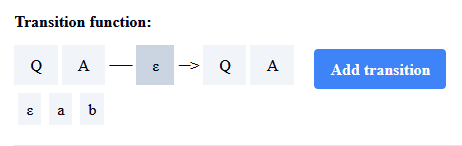
\includegraphics{Figures/PrntScrn_FilledTransition.png}
    \caption{Vyplněný přechod na stránce tvorby zásobníkového automatu}\label{fig:FilledTransition}
\end{figure}

Při kliknutí na tlačítko Save automata ve spodní části stránky se spustí funkce saveEventHandler. Ta jako první zkontroluje, že všechny abecedy mají minimálně jeden symbol a že uživatel vybral počáteční stav a počáteční zásobníkový symbol. Dále zkontroluje, zda se jedná o automat přijímající prázdným zásobníkem nebo přijímajícími stavy a zda je případně vybrán alespoň jeden. Poté ještě zkontroluje, zda je nadefinován alespoň jeden přechod přechodové funkce. Následně se provede kontrola celého zásobníkového automatu pomocí funkce checkPushdownAutomata, která je podrobněji popsána v sekci~\ref{sec:checkPushdownAutomata}. Pokud se nikde nevyskytla chyba, automat se uloží do úložiště a stránka se přepne do simulátoru.

\section{Funkce checkPushdownAutomata pro kontrolu automatu}\label{sec:checkPushdownAutomata}

Poslední důležitou částí implementace je funkce pro kontrolu definice zásobníkových automatů. Tato funkce se volá při nahrání zásobníkového automatu ze souboru nebo při jeho definici přímo na stránce. Funkce postupně prochází jednotlivé části automatu a kontroluje jejich správnost. V případě nalezené chyby si uloží chybovou hlášku a na je všechny vypíše uživateli.

Jako první postupně zkontroluje množinu stavů, vstupní a zásobníkovou abecedu. U všech tří kontroluje, jestli množiny nejsou prázdné a zda neobsahují duplicity. Jelikož typescript neobsahuje datový typ char, ale pouze string, tak u abeced ještě zkontroluje, že všechny symboly jsou délky jednoho znaku.

Dále se kontroluje počáteční stav a počáteční zásobníkový symbol. U obou se zkontroluje, zda jsou součástí konkrétních množin. Pokud automat přijímá množinou přijímacích stavů, tak se pro každý přijímací stav taktéž zkontroluje, zda je součástí množiny stavů. 

Nakonec se kontrolují přechody přechodové funkce. Pro každý přechod se zkontroluje, zda všechny jeho části (oba stavy, zásobníkové symboly a symbol vstupní abecedy, pokud není $\epsilon$) jsou součástí konkrétních množin.

Nakonec se zkontroluje, jestli pole chybových hlášek je prázdné. Pokud není, tak se pomocí funkce alert zobrazí všechny chybové hlášky, viz obrázek~\ref{fig:PDACheckErrors} a funkce vrátí hodnotu false. V opačném případě vrátí funkce hodnotu true.

\begin{figure}[h]
    \centering
    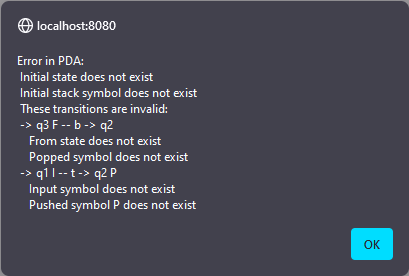
\includegraphics[width=0.6\textwidth]{Figures/PrntScrn_PDACheckErrors.png}
    \caption{Ukázka chybových hlášek kontroly zásobníkového automatu}\label{fig:PDACheckErrors}
\end{figure}

\endinput
\chapter{Uživatelské rozhraní}

Předchozí kapitola~\ref{chap:AppImplemetation} se zabývala převážně funkčností aplikace. V této kapitole se chci zaměřit na to, jak vypadá uživatelské rozhraní a jak aplikace funguje. Kapitola bude rozdělena do několika sekcí, kdy každá sekce se bude věnovat jedné stránce, tomu, co stránka obsahuje a jak se případně ovládá.

\section{Hlavní stránka}

Když si uživatel zobrazí webovou stránku s aplikací, první, co uvidí, je hlavní nabídka. Ta je velice jednoduchá, protože obsahuje nadpis a tři tlačítka vycentrované na středu stránky, obrázek~\ref{fig:UIMainPage}. Každé z techto tlačítek přepne uživatele na stránky, které budou popsané v dalších sekcích této kapitoly:
\begin{itemize}
    \item Tlačítko new --- Stránka pro tvorbu zásobníkového automatu, sekce~\ref{sec:PDABuilder}
    \item Tlačítko upload --- Formulář pro nahrávání zásobníkových automatů, sekce~\ref{sec:UploadForm}
    \item Tlačítko saved --- Výpis úložiště, sekce~\ref{sec:SimulatorPage}
\end{itemize}

\begin{figure}[h]
    \centering
    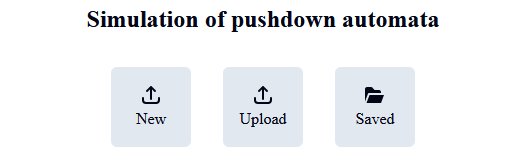
\includegraphics[width=0.8\textwidth]{Figures/PrntScrn_UI_MainMenu.png}
    \caption{Hlavní stránka}\label{fig:UIMainPage}
\end{figure}

\section{Stránka pro tvorbu zásobníkového automatu}\label{sec:PDABuilder}

Po kliknutí na tlačítko new v hlavní nabídce se otevře stránka pro tvorbu zásobníkového automatu. Tato stránka se skládá z několika formulářů a HTML input prvků. 

Jako první je textové pole pro specifikaci názvu automatu. Tento název se pak zobrazuje ve výpisu automatů z úložiště. Dále následuje formulář pro přidávání stavů. Stavy se přidávají po jednom a jejich délka není omezená.D8le následují formuláře pro definování vstupní a zásobníkové abecedy. Symboly se opět přidávají po jednom a jejich délka je omezena na jeden znak. Vstupní pole pro název a formulář pro přidávaní stavů lze vidět na obrázku~\ref{fig:BuilderPart1} včetně chybové hlášky.

\begin{figure}[h]
    \centering
    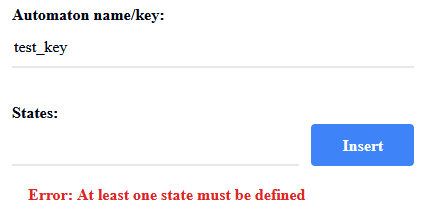
\includegraphics[width=0.5\textwidth]{Figures/PrntScrn_UI_BuilderPart1.png}
    \caption{Název a formulář pro přidávání stavů}\label{fig:BuilderPart1}
\end{figure}

Po těchto třech formulářích následují dva seznamy pro výběr počátečního stavu a počátečního zásobníkového symbolu. Po těchto dvou seznamech následuj část pro určení, zda zásobníkový automat bude přijímat prázdným zásobníkem nebo přijímací stavy. To závisí na tom, zda uživatel zaškrtne zaškrtávacího pole. Pokud zůstane nezaškrtnuté, musí uživatel vybrat alespoň jeden ze stavů níže jako přijímací. Seznam počátečních zásobníkových symbolů a zaškrtávací pole je na obrázku~\ref{fig:BuilderPart2}.

\begin{figure}[h]
    \centering
    
\includegraphics[width=0.5\textwidth]{Figures/PrntScrn_UI_BuilderPart2.png}
    \caption{Seznam počátečních zásobníkových symbolů a zaškrtávací pole pro určení typu zásobníkového automatu}\label{fig:BuilderPart2}
\end{figure}

Poslední část pak slouží k definování přechodů přechodové funkce. Její funkce již byla popsána v sekci~\ref{sec:PDABuilderImplementation}. Jak tato část vypadá lze vidět na obrázku~\ref{fig:FilledTransition}. Pak již následují jen tlačítka na navrácení na hlavní stránku a uložené zásobníkového automatu.

\section{Formulář pro nahrávání zásobníkových automatů}\label{sec:UploadForm}

Druhým tlačítkem v hlavní nabídce se uživatel dostane na stránku s formulářem, který slouží k nahrání zásobníkového automatu ze souboru. Formulář, obrázek~\ref{fig:UploadForm}, je složen ze dvou částí. První je textové pole pro pojmenování automatu. Toto pole se používá jako klíč pro úložiště a zároveň se zobrazuje v výpisu automatů. Pokud je klíč již použitý pro jiný automat, je při odeslání formuláře uživatel dotázán, zda chce automat s tímto klíčem přepsat. Druhé pole pak slouží pro nahrání souboru typu JSON, který obsahuje definici zásobníkového automatu. Při odeslání formuláře se nejprve ze souboru vytvoří instance třídy PushdownAutomata a následně se provede kontrola. Pokud automat nemohl být vytvořen kvůli neodpovídající struktuře nebo obsahuje chyby, je na to uživatel upozorněn společně s výpisem chyb, obrázek~\ref{fig:PDACheckErrors}.

\begin{figure}[h]
    \centering
    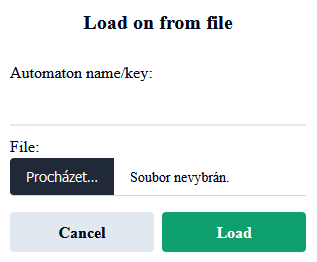
\includegraphics[width=0.45\textwidth]{Figures/PrntScrn_UI_Upload.png}
    \caption{Formulář pro nahrání zásobníkového automatu ze souboru}\label{fig:UploadForm}
\end{figure}

\section{Výpis úložiště}\label{sec:StoragePage}

Třetím tlačítkem v hlavní nabídce si uživatel může zobrazit seznam všech automatů, které jsou uložené v úložišti. Vzhled této stránky je na obrázku~\ref{fig:Storage}. Nad samotnou tabulkou je nadpis a tlačítko pro návrat do hlavní nabídky. Samotná tabulka pak má 6 sloupců a každý řádek odpovídá jednomu automatu v úložišti.

První sloupec obsahuje název automatu, dalších 5 sloupců pak obsahuje tlačítka. První tlačítko zobrazí stránku, na které je tabulka s informacemi o automatu. Druhé tlačítko přepne uživatele na stránku pro tvorbu zásobníkového automatu, kde může uživatel automat zeditovat. Třetí tlačítko přepne uživatel na stránku simulátoru, která je popsána v podkapitole~\ref{sec:SimulatorPage}, a nastaví tam konkrétní zásobníkový automat. Čtvrté tlačítko pak slouží pro stažení automatu jako soubor typu JSON.@ Poslední tlačítko pak slouží pro vymazání automatu z úložiště.

\begin{figure}[h]
    \centering
    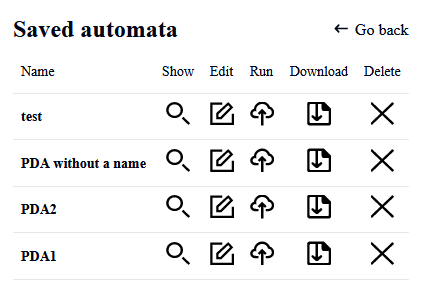
\includegraphics[width=0.5\textwidth]{Figures/PrntScrn_UI_Storage.png}
    \caption{Výpis automatů v úložišti}\label{fig:Storage}
\end{figure}

\section{Simulátor}\label{sec:SimulatorPage}

Poslední stránkou této aplikace je stránka samotného simulátoru. Na tuto stránku se může uživatel dostat třemi způsoby:

\begin{itemize}
    \item Vytvořením automatu na stránce popsané v podkapitole~\ref{sec:PDABuilder}
    \item Nahráním automatu ze souboru
    \item Vybráním automatu z úložiště
\end{itemize}

Při zobrazení této stránky je jako první otevře modální okno pro zadání vstupu, které je na obrázku~\ref{fig:TapeInput}. Po potvrzení vstupu se okno schová a uživatel vidí již samotný simulátor. Na obrázku~\ref{fig:Simulator} lze vidět stránku v průběhu simulace.

\begin{figure}[h]
    \centering
    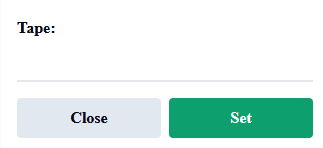
\includegraphics[width=0.4\textwidth]{Figures/PrntScrn_UI_TapeInput.png}
    \caption{Okno pro zadání vstupu}\label{fig:TapeInput}
\end{figure}

Samotný simulátor se pak skládá z několika částí. V horní částí je řádek, který symbolizuje vstupní pásku se symboly. Symboly s tmavším pozadím je symbol, který bude přečten jako další. Nalevo od něj jsou již přečtené symboly a napravo symboly ještě nepřečtené. Na pravé straně se pak nachází zásobník. Symbol, který se nachází nejvýše a má tmavší pozadí, je symbol na vrcholu zásobníku, takže bude přečten v dalším kroku. 

Na levé straně stránky se nachází tři oblasti seřazené ve sloupci. První oblast, která se nachází nejvýše, zobrazuje aktuální stav, ve kterém se nachází řídící jednotka. Ve druhé oblasti, která je na obrázku~\ref{fig:Simulator} prázdná, se zobrazují možnosti volby dalšího přechodu u nedeterministických zásobníkových automatů. Příklad volby je na obrázku~\ref{fig:TransitionFunctionChoosing}. Třetí část pak obsahuje ovládací prvky simulátoru. Tlačítko Close simulation ukončí simulaci a vrátí uživatele do hlavní nabídky. Set new tape otevře modální okno pro zadání vstupu, stejně jako při prvním otevření stránky.
Šipky pak slouží k samotnému ovládání simulace. Šipky na krajích slouží ke spuštění automatické simulace, šipky uvnitř pak slouží k manuálnímu krokování. Tlačítko uprostřed slouží k pozastavení simulace. Posledním ovládacím prvkem je posuvník, který slouží k nastavení času mezi jednotlivými kroky při automatické simulaci.

Poslední částí simulátoru je místo uprostřed obrazovky, které slouží k zobrazování informací. V horní částí jsou dvě tlačítka, které přepínají, co bude zrovna zobrazeno. Levé tlačítko slouží k zobrazení tabulky s definicí aktuálně používaného zásobníkového automatu, levé pak slouží k zobrazení historie přechodů již použitých v této simulaci.

\begin{figure}[h]
    \centering
    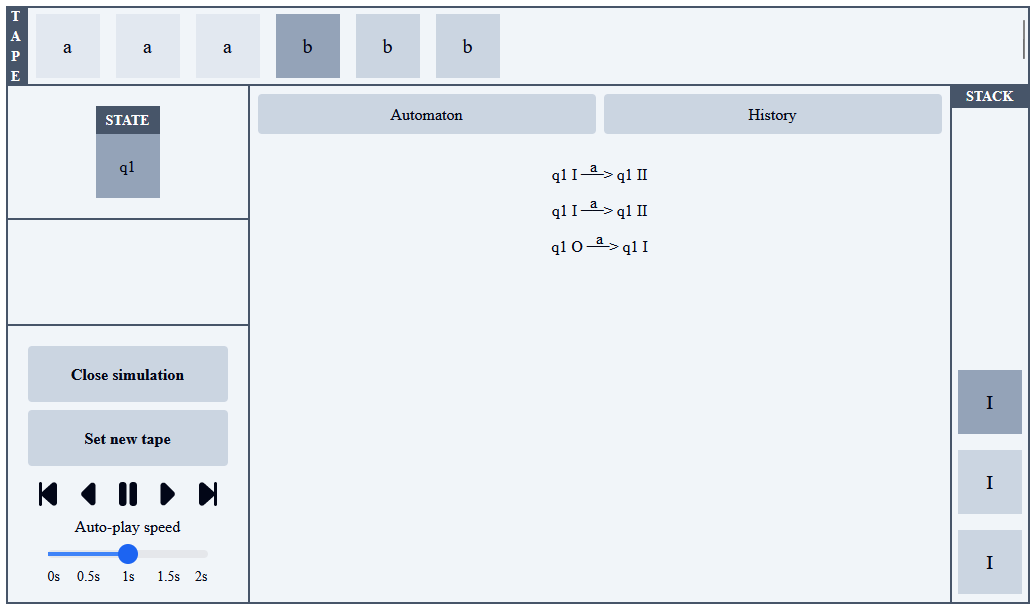
\includegraphics[width=\textwidth]{Figures/PrntScrn_UI_Simulator.png}
    \caption{Okno pro zadání vstupu}\label{fig:Simulator}
\end{figure}

Aplikace podporuje i zobrazení na menších obrazovkách, jako mají například telefony nebo tablety. Toto zobrazení se oproti tomu na obrázku~\ref{fig:Simulator} liší ve dvou věcech --- vstupní páska je svisle na levé straně obrazovky a středová část s informacemi je jako modální okno, které se otevírá tlačítkem.

\endinput
\chapter{Závěr}\label{chap:Conclusion}

Cílem této práce bylo vytvořit aplikaci, která by uživateli umožňovala graficky simulovat činnost zásobníkových automatů. Jako první bylo nutné si ale nastudovat problematiku zásobníkových automatů, jak jsou definovány, jaké jsou jejich typy a jak fungují. Poté jsem vytvořil webovou aplikaci, dovoluje uživateli simulovat činnost libovolného zásobníkového automatu pro jím zadaný vstup. Zásobníkové automaty může uživatel nahrát jako soubor nebo je vytvořit přímo v aplikaci. Všechny zásobníkové automaty se ukládají do lokálního úložiště prohlížeče, aby k nim měl uživatel přístup a při příštím spuštění aplikace. Následně jsem vytvořil několik vzorových zásobníkových automatů, na kterých jde vidět činnost aplikace a pomocí kterých jsem aplikaci testoval.

Práci je možné v budoucnu rozšířit a další funkce, jako je např.\ možnost převodu mezi automaty přijímajícími prázdným zásobníkem a přijímajícími stavy, grafické zobrazení automatu nebo možnost vytvoření zásobníkového automatu z bezkontextové gramatiky.
\endinput

% Seznam literatury
\printbibliography[title={Literatura}, heading=bibintoc]

% NOTE: Přílohy
% Prilohy
\appendix

\end{document}
